	\begin{figure}[h]
	\centering
		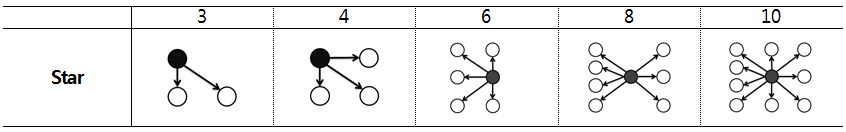
\includegraphics[height=50pt]{Topologies_Star}
		\caption{Bayesian Network Topologies : Star}
	\end{figure}	
	
	% Star 형태는 한 개의 node가 여러 개의 자식 node를 가진 형태를 말한다.
	If one node has plurality of child node, then this form called Star.

\begin{figure}[!bhp]
	\centering
		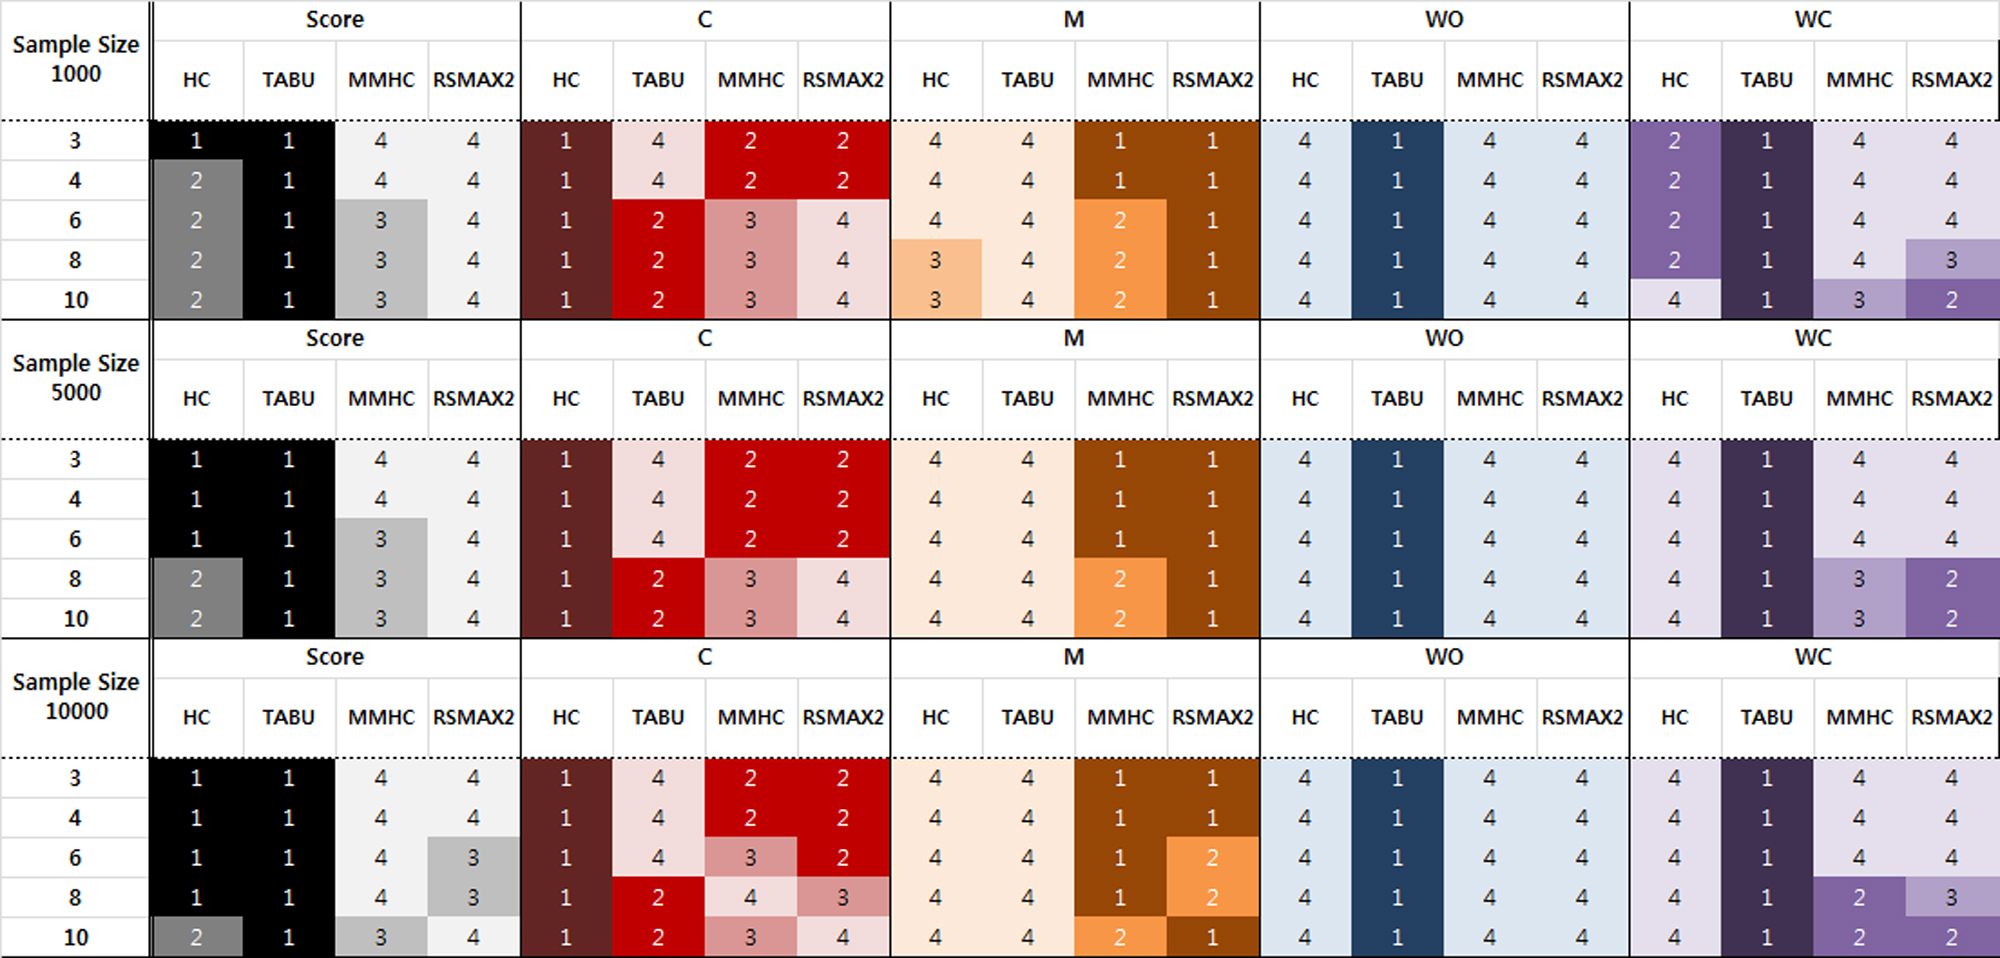
\includegraphics[height=155pt]{Result_Star}
		\caption{Summary for Comparison via Star}
	\end{figure}	

% Star 역시, 알고리즘별 성능이 크게 차이가 발생하지 않았다.
Star also, the performance of each algorithm was not different significantly occurs.

% Score 기준으로 비교했을 때는 TABU search가 좋은 성능을 보여주었지만, 목표 네트워크와 학습 네트워크를 비교했을 경우, 상대적으로 Hill-climbing이 line 형태에서 좋은 성능을 보여주었다.
When compared by score, TABU search is good then the other algorithms. But when compared to between the target network and learning network, Hill-climbing showed good performance relatively for the line form.

% 특이한 점은, node 개수가 작을 때, TABU search는 score에 따른 성능이 좋음에도 불구, 다른 알고리즘에 비해 C의 개수가 압도적으로 적고, M, WO, WC의 개수가 무척 높은 모습이 나타났다. 그러나 node 개수가 많아질수록, sample size가 커질수록 다른 알고리즘에 비해 C의 개수가 많아지고, M, WO, WC의 개수가 줄어드는 현상이 나타났다.
Specific point, when the node number is small, TABU search despite the good performance by score, but the number of C is overwhelmingly smaller than the other algorithms. And M, WO and WC is very large. However, as the number of node increases, becoming the number of C is increased, and M, WO, WC is decreases.

% 그럼에도 불구하고 Hill-climbing의 성능에 미치지는 못하였다.
And yet, did not win to the performance of Hill-climbing.

% 모든 알고리즘이,Sample size가 커짐에 따라 WO, WC 개수가 크게 줄어드는 모습이 나타났다.
All algorithms while sample size increases, WO and WC is greatly reduced.
	
	\begin{figure}[p]
	\centering
		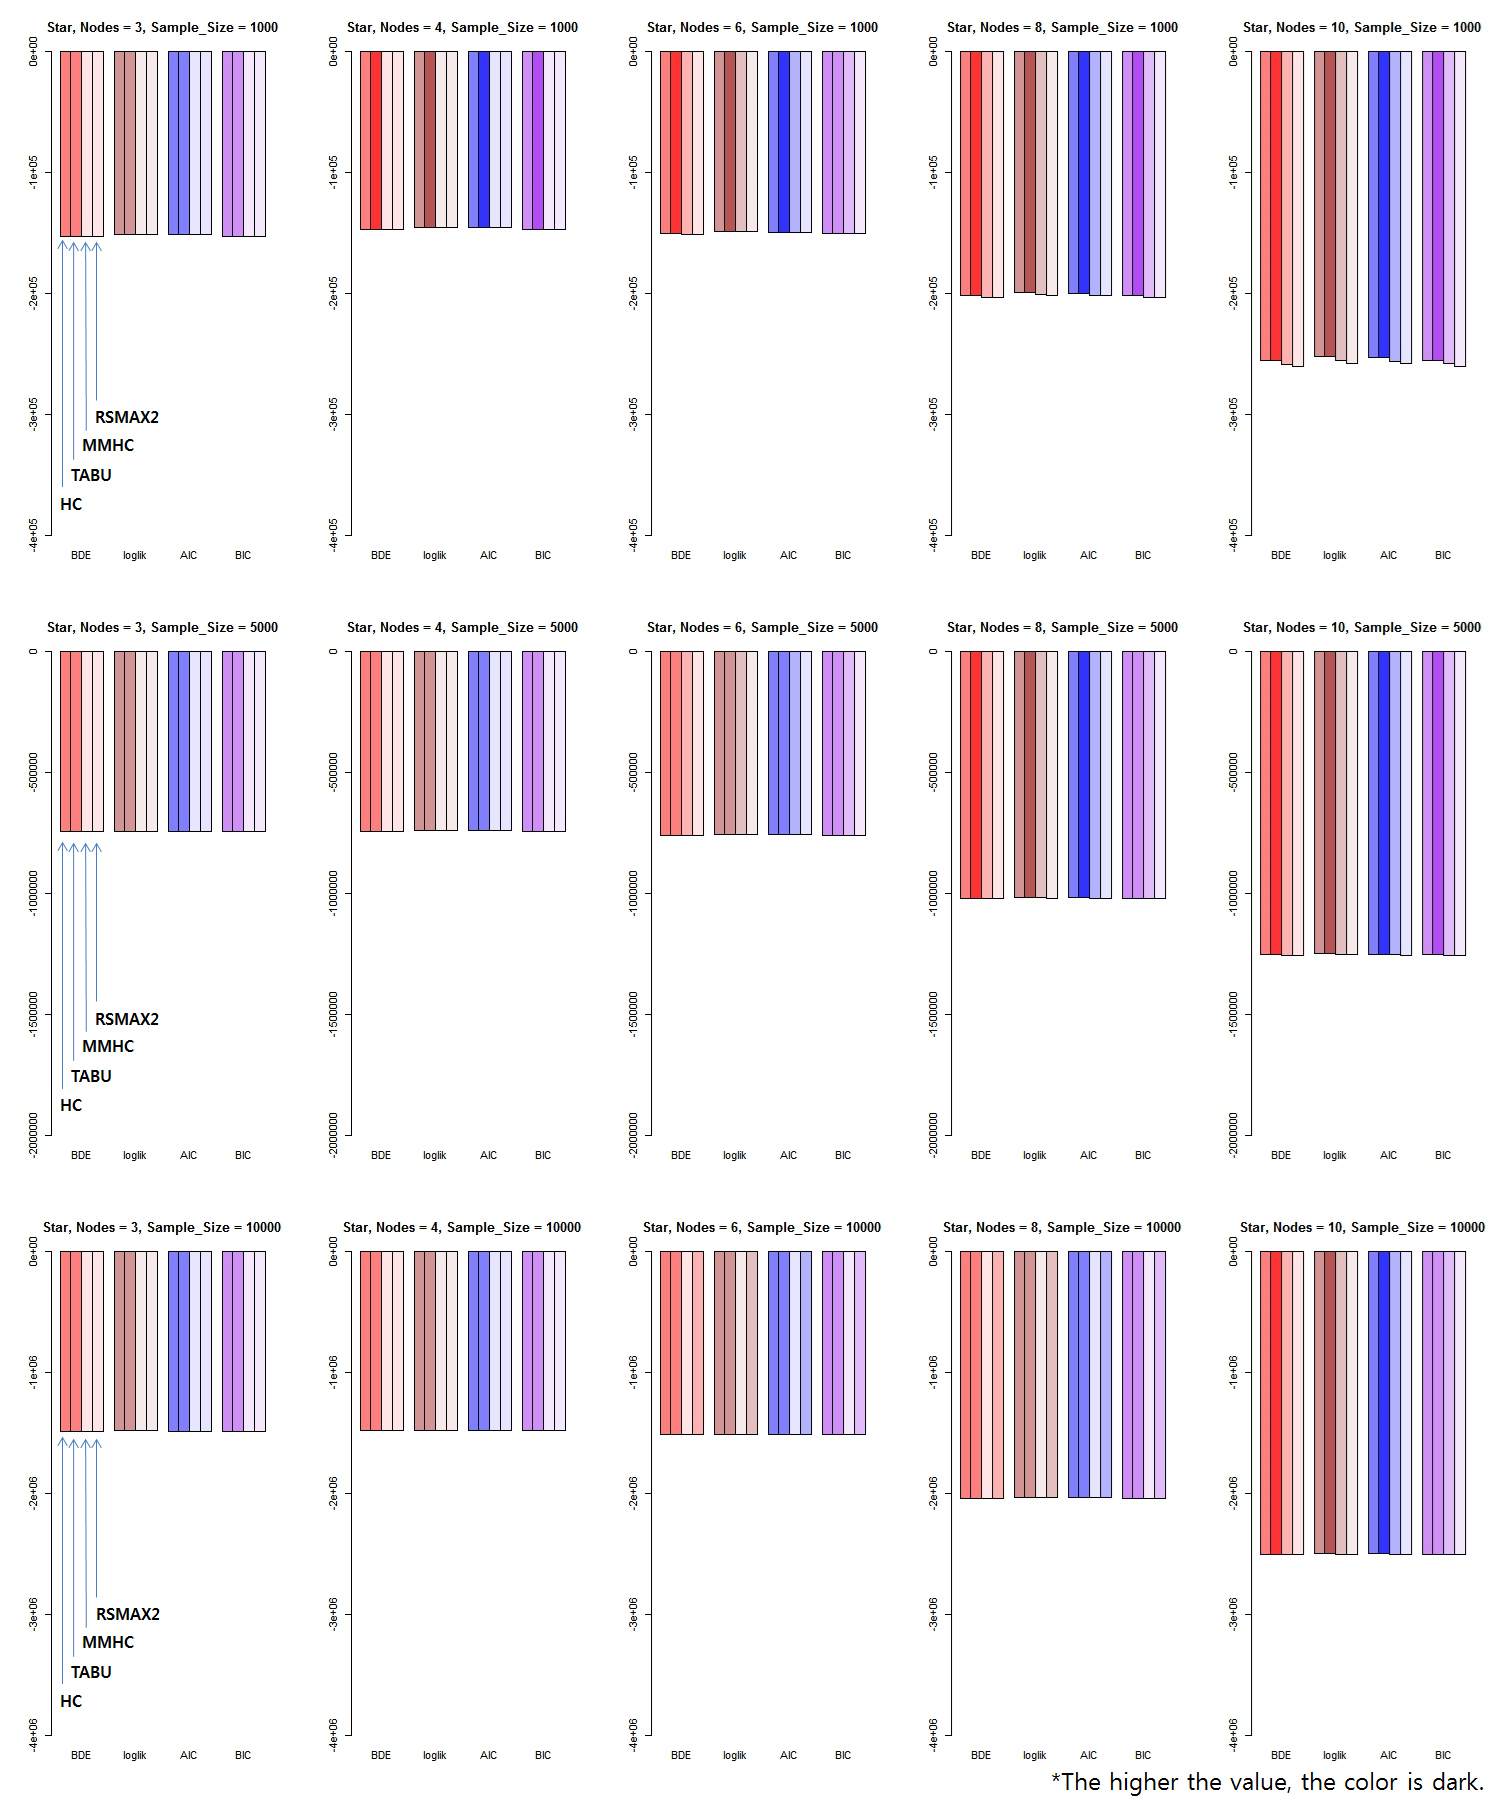
\includegraphics[height=500pt]{03_Star_Score}
		\caption{Comparison of scores via Star}
	\end{figure}	

	\begin{figure}[p]
	\centering
		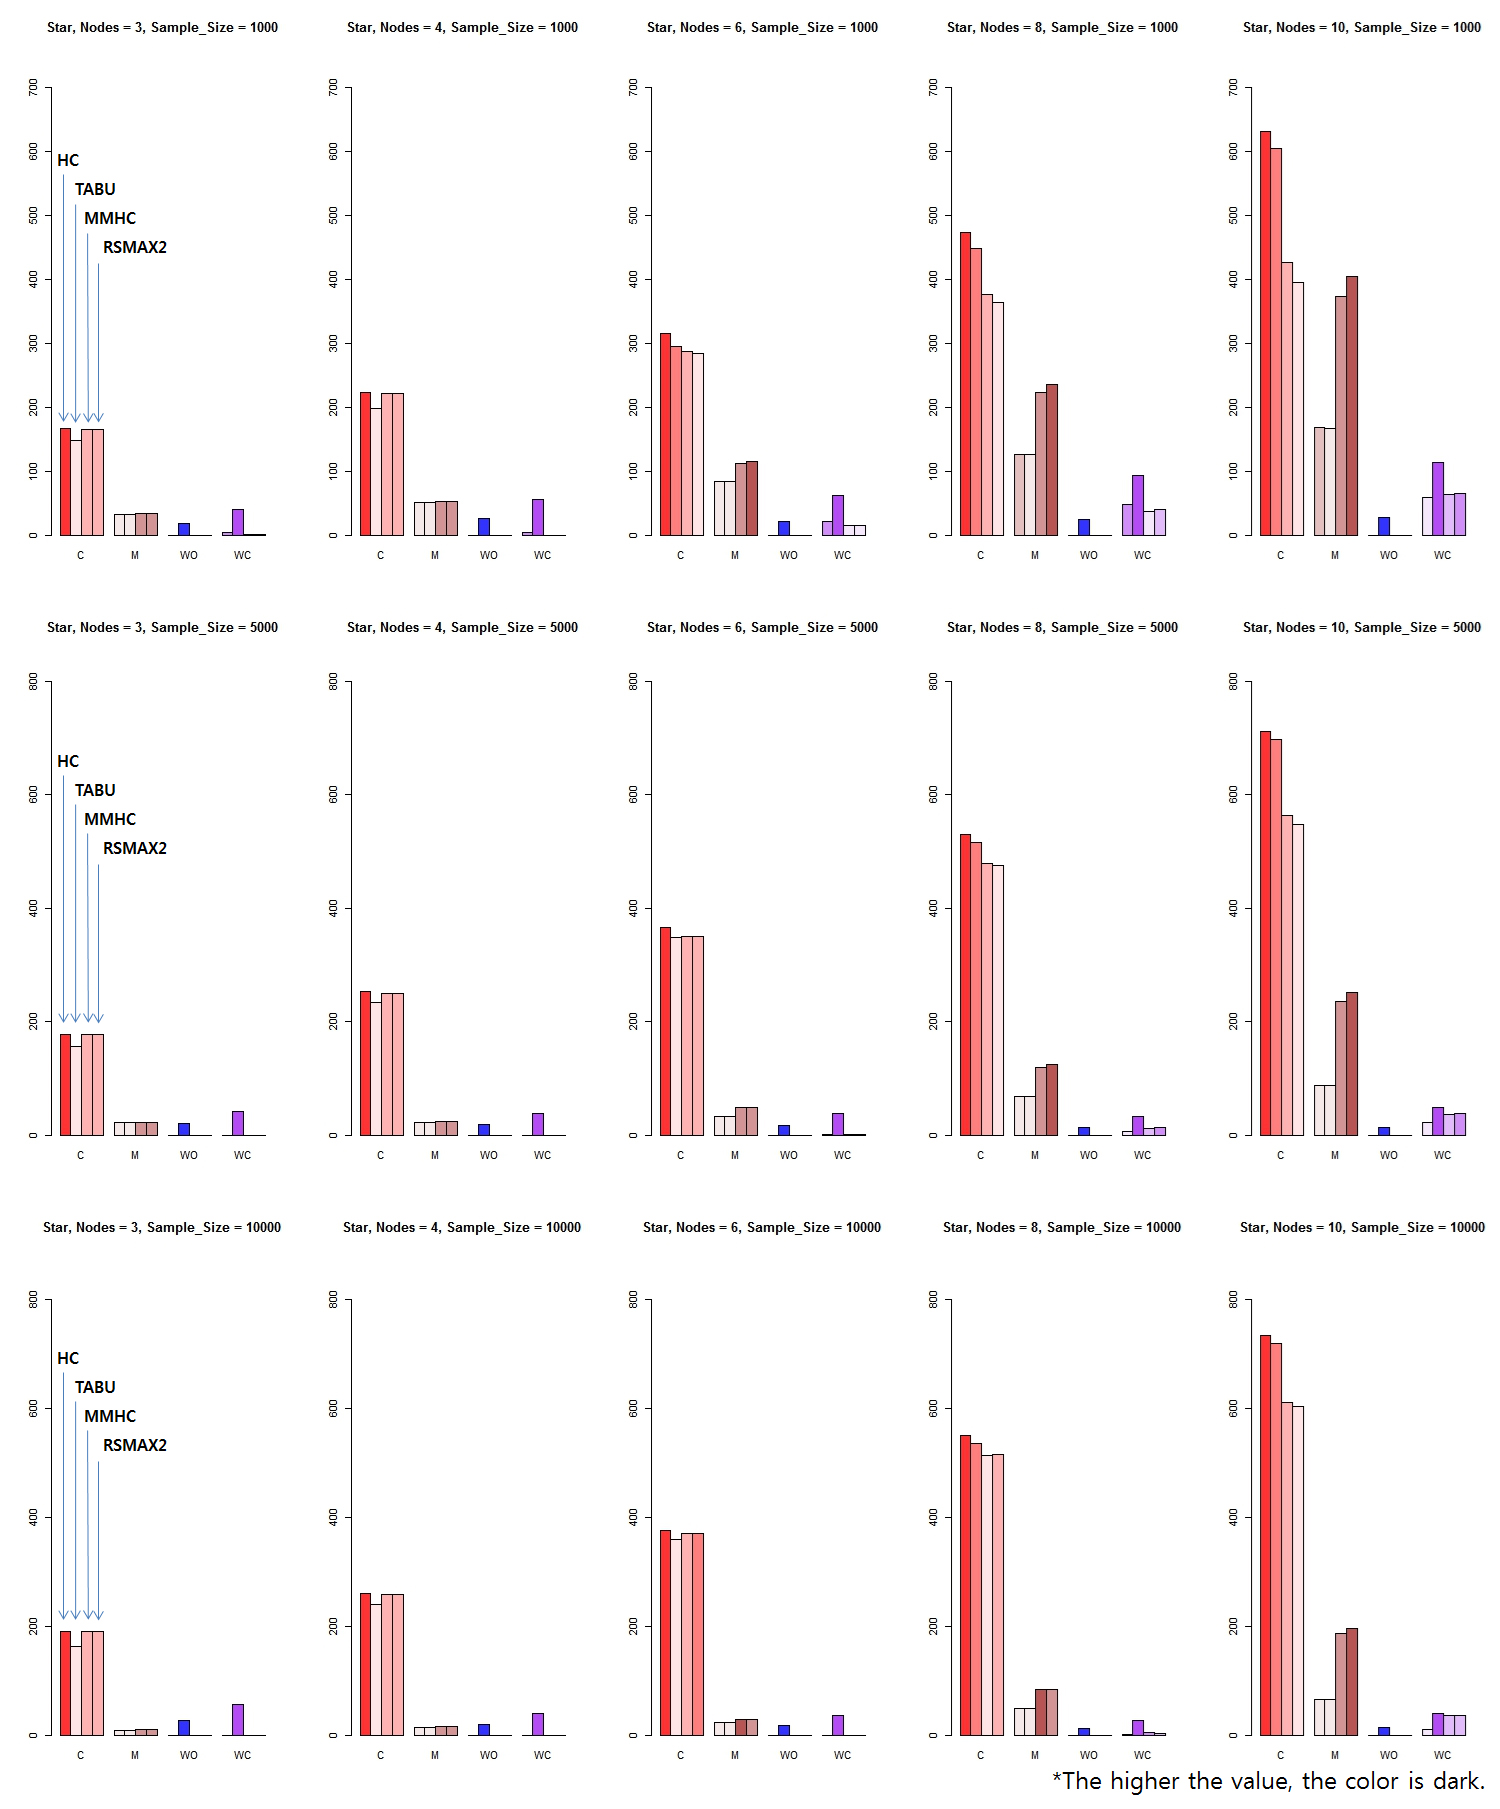
\includegraphics[height=500pt]{03_Star_Arcs}
		\caption{Comparison of correct arcs via Star}
	\end{figure}	
